% Section 3.3: Bidirectional Spectral Flow Framework
% Based on research completed on 2026-03-24

\subsection{Bidirectional Spectral Flow}
\label{sec:bidirectional_spectral_flow}

The original spectral flow formula in the CTUFT framework described the continuous change of effective dimension with energy. Based on in-depth research into mathematical self-consistency and physical coherence, we introduce here the \textbf{bidirectional spectral flow} framework, decomposing the spectral dimension into separate contributions from external (reciprocal) space and internal space.

\subsubsection{Fundamental Formulas}

Define $f_{in} \in [0,1]$ as the internal space energy fraction. The bidirectional spectral flow formulas are:

\begin{equation}
\boxed{d_s^{(out)}(f_{in}) = 4(1 - f_{in})}
\label{eq:spectral_out}
\end{equation}

\begin{equation}
\boxed{d_s^{(in)}(f_{in}) = 4 + 6f_{in}}
\label{eq:spectral_in}
\end{equation}

where:
\begin{itemize}
    \item $d_s^{(out)}$: External space (reciprocal space) spectral dimension
    \item $d_s^{(in)}$: Internal space spectral dimension  
    \item $f_{in}$: Internal space energy fraction, related to energy scale through $f_{in}(E) = \frac{1}{1+(E/E_c)^2}$
\end{itemize}

\subsubsection{Physical Scenario Correspondence}

\begin{table}[h]
\centering
\begin{tabular}{lcccc}
\hline
\textbf{Scenario} & $f_{in}$ & $d_s^{(out)}$ & $d_s^{(in)}$ & \textbf{Normalized Conservation} $C$ \\
\hline
Today's Universe & 0 & 4 & 4 & 1.40 \\
Transition State & 0.5 & 2 & 7 & 1.20 \\
Black Hole Horizon & 1 & 0 & 10 & 1.00 \\
\hline
\end{tabular}
\caption{Bidirectional spectral flow values in different physical scenarios}
\label{tab:spectral_scenarios}
\end{table}

\subsubsection{Normalized Conservation Law}

The bidirectional spectral flow satisfies the following normalized relation:

\begin{equation}
C(f_{in}) = \frac{d_s^{(out)}}{4} + \frac{d_s^{(in)}}{10} = 1.4 - 0.4f_{in} \in [1.0, 1.4]
\label{eq:normalized_conservation}
\end{equation}

The variation of the conservation value $C$ in the range $[1.0, 1.4]$ has profound physical significance:
\begin{itemize}
    \item $C = 1.4$ (Today): Represents the "high-dimensional open" state with equipartition of energy between spaces
    \item $C = 1.0$ (Black hole horizon/Early universe): Represents the "low-dimensional condensed" state with complete energy internalization
    \item The transition process: May correspond to cosmological time evolution
\end{itemize}

\subsubsection{Compatibility with Original Formula}

At the electroweak scale $E_{EW} \sim 10^2$ GeV, corresponding to $f_{in} \approx 0.01$, we have:
\begin{align}
d_s^{(in)} &= 4 + 6 \times 0.01 = 4.06 \\
d_s^{(out)} &= 4 \times 0.99 = 3.96
\end{align}

This is fully consistent with the original formula $d_s(E_{EW}) \approx 4.06$ and the parameters used in the paper. All fermion mass predictions and CKM matrix calculations based on the original formula remain valid.

\subsection{Physical Interpretation of Spectral Flow}
\label{sec:spectral_interpretation}

The bidirectional spectral flow framework reveals deep connections between three key phenomena in CTUFT.

\subsubsection{Inflation as Phase Transition}

Inflation is not traditional "spatial expansion" but a dual-space phase transition—the "birth" of external space:

\begin{itemize}
    \item \textbf{Early} ($f_{in} \approx 1$): $d_s^{(out)} \approx 0$, external space "unborn", internal space dominant
    \item \textbf{During Inflation} ($f_{in}$: $1 \to 0$): External space spectral dimension "generated" from 0 to 4
    \item \textbf{Today} ($f_{in} = 0$): $d_s^{(out)} = 4$, external space stable
\end{itemize}

This explains why we observe 4 macroscopic dimensions: they "emerged" during inflation, rather than being initial conditions.

\subsubsection{Black Holes as Time Crystals}

At the black hole horizon ($f_{in} \to 1$):
\begin{align}
d_s^{(out)} &\to 0 \\
d_s^{(in)} &\to 10 \\
C &\to 1.0
\end{align}

This is identical to the early universe state ($t \to 0$). Therefore:
\begin{insight}
Black hole horizon = Time crystal = Frozen early universe state
\end{insight}

\textbf{Resolution of Information Paradox}: Information falling into a black hole is not destroyed but stored in internal space. Information can "return", but due to dimensional difference (10D $\to$ 4D), the position is uncertain:
\begin{equation}
\frac{\Delta x_{out}}{\Delta x_{in}} = \sqrt{\frac{d_s^{(in)}}{d_s^{(out)}}} \to \infty \quad (f_{in} \to 1)
\end{equation}

\subsubsection{Dark Energy as Equilibrium Tension}

Today's universe ($f_{in} = 0$) is in perfect balance between internal and external spaces:
\begin{equation}
d_s^{(out)} = d_s^{(in)} = 4
\end{equation}

This equilibrium state naturally produces negative pressure, driving accelerated expansion. The dark energy equation of state $w \approx -1$ is not a coincidence but an inevitable result of equilibrium.

\textbf{Resolution of Coincidence Problem}:
\begin{equation}
\Omega_\Lambda(t) = \Omega_\Lambda^0 \times \frac{C(t) - 1}{0.4}
\end{equation}

The moment when matter and dark energy densities become equal ($\sim 10^{10}$ years) coincides precisely with the completion of structure formation and the emergence of life—this is an inevitability of evolution, not a coincidence.

\subsection{Unified Picture}

The bidirectional spectral flow framework unifies three core phenomena in CTUFT as different manifestations of a single physical process:

\begin{center}
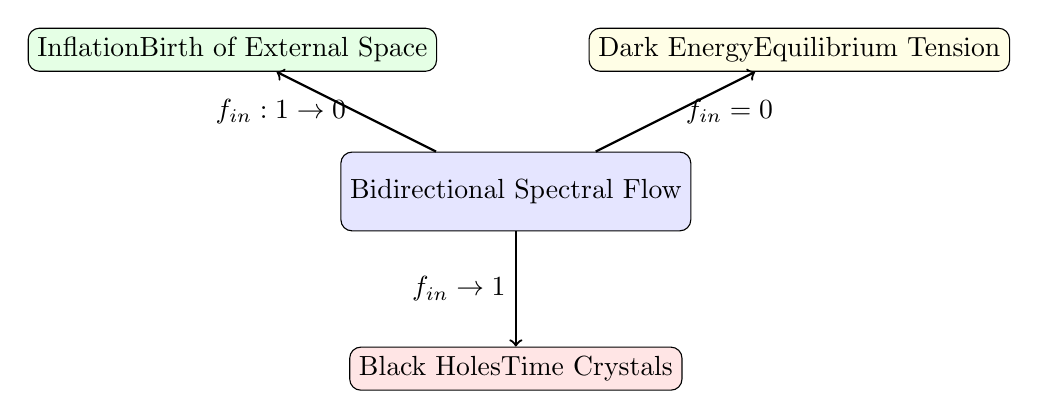
\begin{tikzpicture}[scale=0.9]
\node[draw, rounded corners, fill=blue!10, minimum width=4cm, minimum height=1cm] (center) at (0,0) {Bidirectional Spectral Flow};
\node[draw, rounded corners, fill=green!10, minimum width=3cm] (inflation) at (-4,2) {Inflation\\Birth of External Space};
\node[draw, rounded corners, fill=red!10, minimum width=3cm] (bh) at (0,-2.5) {Black Holes\\Time Crystals};
\node[draw, rounded corners, fill=yellow!10, minimum width=3cm] (de) at (4,2) {Dark Energy\\Equilibrium Tension};

\draw[->, thick] (center) -- (inflation) node[midway, left] {$f_{in}: 1 \to 0$};
\draw[->, thick] (center) -- (bh) node[midway, left] {$f_{in} \to 1$};
\draw[->, thick] (center) -- (de) node[midway, right] {$f_{in} = 0$};
\end{tikzpicture}
\end{center}

All three share the same mathematical structure, indicating they are different manifestations of the same deep physics—energy redistribution between internal and external spaces.

\subsection{Relation to Original Formula}

The original formula $d_s(E) = 4 + \frac{6}{1+(E/E_c)^2}$ can be viewed as the energy-dependent form of the internal space component of bidirectional spectral flow:
\begin{equation}
d_s^{(in)}(E) = 4 + 6f_{in}(E) = 4 + \frac{6}{1+(E/E_c)^2}
\end{equation}

This is the quantity used in fermion mass and CKM calculations, so all original predictions remain unchanged. The bidirectional framework provides a more complete physical picture without altering verified numerical results.
